% #####################################################
% #####################################################
% #####################################################
\setchapterpreamble[u]{\margintoc}
\chapter{Vacuum RF Breakdown and Multipactor}\label{chap:Multipactor}

\epigraph{There is all the difference in the world between knowing about and knowing how to do.}{James Evans, The History and Practice of Ancient Astronomy}

\marginnote{Parts of this chapter are taken from \citeauthyear{hillairet2017} and from the PhD of Nicolas Fil and Adrien Plaçais and their associated publications \cite{fil2016, fil2017, fil2017-2,fil2018, placais2018,  placais2019}. These PhDs have been supervised in collaboration between CNES, ONERA and CEA since 2014.}

\section[RF Breakdowns]{RF Breakdowns and Vacuum Arcs}
RF breakdowns and vacuum arcs are a recurrent problematic in high RF power applications and magnetic nuclear fusion experiments make no exception. A \textit{vacuum arc} can be defined as an electric discharge occurring between two electrodes in vacuum \sidecite{Timko2011}. In the context of RF heating and current drive for tokamaks, electrical \textit{breakdown} almost always means a vacuum arc affecting RF systems performances. In this manuscript, both terms are used with the same meaning.

ICRH and LHRF systems have general concerns with voltage limitations, in particular \sidecite{bobkov2003, goniche2014}:
\begin{itemize}
	\item between metallic electrodes of coaxial lines,
	\item between waveguide walls of (thin) rectangular waveguides,
	\item with dielectric elements of vacuum feed-throughs,
	\item inner conductor mechanical supports
\end{itemize}
These parasitic phenomenon can limit the power transmitted from the RF sources to the plasma.

\subsection{Formation Mechanisms}

Despite the enormous number of papers published on this topic, some uncertainty remains about breakdown overall processes. This uncertainty is due to the fact that few mechanisms are (or seem) to be involved \sidecite{insepov2011-1}. Moreover, they occur on very short time scales \sidecite[+0.5cm]{zhou2019}, during which experimental parameters vary over 12 orders of magnitude \cite{Timko2011}. As setup are often unique and results delicate to compare for an application to another, few dedicated experimental studies have been conducted to explore different  experimental parameters relevant to tokamak antennas \sidecite{bobkov2003, Graves2006a, becerra2007, dinca2009}.

It is know since some time that DC breakdown mechanism under ultra-high vacuum is related to local breakdown fields which mostly depend on the electrode materials \sidecite{alpert1964, descoeudres2009}. Recent experimental and modelling works performed for accelerators argue that arcing can be explained by the properties of surface cracks and \textit{unipolar arcs}\sidenote[][+1cm]{unipolar arcs (or cathodic arcs) are similar to vacuum arcs, only instead of striking between two solid electrodes they strike between one solid electrode and a plasma\cite[§9.8]{wesson2011}.} and explained from the following steps \sidecite{insepov2013}:
\begin{enumerate}
\item An initial mechanical failure/cracks of the surface due to fatigue, producing detached fragments,
\item high external electric field is applied, locally enhanced at the failure/cracks location (known as \textit{emitters})
\item Electrons extracted from secondary or field emission further ionize these fragments,
\item A local plasma is initiated, controlled by the plasma sheath and material properties. 
\item The plasma density increases exponentially up to some equilibrium state, during which local temperature increases due ion bombardment/current hitting the wall, eventually melting it. Ion induced sputtering is a source of additional ions for the plasma.
\item Additional surface damages are produced by the arc (due to heating, melting then cooling), which can further initiate new arcs.
\end{enumerate}
If the energy source that gave birth to the arc is not stopped, the arc can continuously burn. Unipolar arcs can travel on the surfaces of the cathode (negatively charged), as the emitter spot is constantly changing. In the absence of a magnetic field, the spot "movement" can be described with a random-walk model\sidecite{daalder1983}. In the presence of a magnetic field $\Bbf_0$, the spot follows a retrograde motion in the $-\jbf\times\Bbf_0$ direction\sidecite{wesson2011}. 

As noted in the step 3, both field emission and secondary emission have been identified as the main mechanism leading to increase the electron population, which further cause ionization and electron avalanche \sidecite{hohn1997}. The leading cause depends of the geometry and the RF frequency at play. 

It is generally admitted in the fusion community that \textit{field emission} is the main mechanism limiting ICRF power while it is mostly  \textit{secondary emission} triggered by \textit{multipactor} effect for LHRF \sidecite{goniche2014, wukitch2004}. Field emission is an electron tunnelling effect induced by an electric field. Secondary emission is a phenomenon where primary incident particles of sufficient energy, when hitting a surface or passing through some material, induce the emission of secondary particles, mostly electrons called \textit{secondary electrons}. However, multipactor also affect ICRF systems, generally at relatively low power/voltage, but can also lead to breakdowns. Work on multipactor for ICRF and LHRF are detailled in Section~\ref{sec:multipactor_icrf} and Section~\ref{sec:multipactor_lhrf}. Because multipactor is affecting satellite payloads, a collaboration between CNES and ONERA has been initated in 2004 and some results are presented in the Sections TODO.



\subsection{Arc Detection}
Breakdowns appearing in RF system can induce changes on the effective impedance which may detune the matching system and allows reflected power to return to the RF sources. Thus, reflection coefficient is the primary breakdown detection method in both ICRF and LHRF. However, if the breakdown is close to a voltage node, the VSWR or reflection coefficient’s phase may be almost unperturbed while increasing the apparent power coupling \sidecite{monakhov2007, goniche2014}. It is thus of great importance to detect these breakdowns as well as to switch-off sources to avoid damages. 

Additional detection techniques such as Sub-Harmonic Arc Detection (SHAD) \sidecite[-0.5cm]{dinca2011}, Scattering Matrix Arc Detection (SMAD) \sidecite{vrancken2009} or optical detection have been implemented or proposed in various systems to complete reflection coefficient method \sidecite{dinca2009, bosia2011}. 



% #######################################################
\section[Multipactor]{Multipactor in High Power RF Devices}
Multipactor is a process by which electron population increases from a resonant \textit{secondary emission} multiplication inside an RF device operating under vacuum conditions. It was first recognized and described by \citeauthyear{farnsworth1934} for the purpose of electron multiplication in vacuum tubes. The electron population increases if both criteria are met\sidecite{vaughan1988}: 
\begin{itemize}
	\item A Secondary Emission Yield (SEY)\sidenote{The SEY is the number of secondary electrons emitted per incident electron impacting a material surface.} higher than one,
	\item A synchronism of the electron motion between electrodes with the RF electric field.
\end{itemize}

In high power RF devices under vacuum, this phenomenon is usually not desirable, since it can detune RF systems or ultimately lead to an avalanche effect and the development of a discharge which can damage RF components, even at pressures two order of magnitude below Paschen breakdown limit \sidecite[-1cm]{kishek1998, graves2006}. As it concerns RF system in vacuum environment, it affects satellite payloads\sidecite{rozario1994, anzahormigo2014}, particle accelerators \sidecite[+0.7cm]{elkhaldi2019} and of course fusion experiments. When not detected quickly enough, local plasma can be initiated by multipacting electrons and finally to an arc \sidecite[-0.3cm]{hohn1997}. These arcs can lead to surface erosion \sidecite{goniche2012}, dielectric components metallization \sidecite{wang2015} or water/air leaks due to punctured components such as bellows or vacuum windows \sidecite{neuber1998, neuber2007}. 

%The ICRF and LHRF antennas are  made of copper or silver-coated stainless-steels structures and are located in vacuum environments. The vacuum sealing with pressurized transmission lines is made with the help of ceramics such as alumina, aluminium nitride, beryllium oxide or diamond. 

Signature of multipactor breakdowns have been found to be low amplitude and wideband spectrum of excited frequencies at the opposite behaviour than high voltage arcs \cite{dinca2009}. Voltage handling limits also arise in the antenna facing the plasma, which also reduce the ultimate antenna coupled power. Impurity production, increasing the neutral particles pressure, degrades the antenna voltage handling. Experimental works identified multipactor as the leading explanation for observed ICRF antenna neutral pressure limit \sidecite{graves2006}.

In some cases however, multipactor-induced discharges can be desired for vacuum RF conditioning \sidecite{mishra2010}. In addition to standard cleaning procedures, surface conditioning is necessary to increase the voltage handling capability. To this end, short low power (1-10~kW) RF pulses (100-1000~ms) are applied on RF antennas under vacuum (no plasma) to reduce the secondary emission of the metallic surfaces\sidecite{halbritter1982}. This method, used both in ICRF \sidecite[+0.5cm]{colestock1985, wang2015} and LHRF \sidecite[+1.5cm]{ekedahl1998,goniche2012} is an essential preliminary step before increasing both power and duration to medium values (10-100~kW/100-200~ms) in order to increase the surface temperature due to RF losses and make them out-gass (still in vacuum). Once done, RF commissioning on plasma at medium powers and durations can be realized to clean parts of the antenna that do not carry a substantial fraction of the current \sidecite{noterdaeme1993}, before finally achieved high voltage conditioning at high power (>100kW/10ms) to further increase the voltage stand-off limit.

In addition, magnetic fusion RF heating and current drive systems are subjected to the high magnetic field environment of the experiments in the Tesla range. The presence of magnetic field affects obviously the electron trajectories and thus the multipactor resonances. During the PhD of Nicolas Fil \sidecite{fil2017-1}, he has measured that magnetic field also modify the secondary emission characteristics of a metal, which further impact multipactor processes. 

Finally, dielectric are also subject to multipactor, which can be critical when these dielectric are safety components such as vacuum feed-through/windows. Because they are not conductor per definition, dielectrics can accumulate electric charges at their surface. The dynamics of this accumulation can further modify multipactor discharges \sidecite{sorolla2017}. This aspect has been studied during the PhD of Adrien Plaçais \sidecite{placais2020}.


\subsection{Multipactor in ICRF}\label{sec:multipactor_icrf}
In coaxial geometries, multipactor-induced breakdown disappear when the power level is above few kilowatts \sidecite[-0.5cm]{woo1968, woo1970}, which is a typical signature of multipactor resonance as expected from theory  \sidecite{udiljak2007, semenov2007, becerra2007}. The later exact power level depends on the RF system such as $Q$-factor and transmission line dimensions and the materials used. The Figure~\ref{fig:powerthresholdcoax} illustrates the multipactor power threshold versus the line impedance as calculated in a coaxial geometry with a fixed outer diameter at 50~MHz. Such breakdowns are known to happen when the power builds up during the start-up phase of the generators. For this reason, the RF rise time is generally set as short as possible, in order to exceed this power window as fast as possible (“push-through”) and to be faster than the multipactor rise time \sidecite{graves2006, kishek1997, mishra2010}. In practice, the maximum current drawn by the generator or the RF power feedback systems limits this rise time to no more than typically 50~µs/kW, which is generally sufficient to avoid multipactor during power ramp-up. 

%Simulation of multipactor in a 30 Ohm coaxial line of dimensions (Dint/Dext=140/230 mm) indicates that the number of initial seed electrons is doubled within 60-200 ns when RF power is below 2 kW (Fig. 2, right)


\begin{figure}[h]
	\centering
	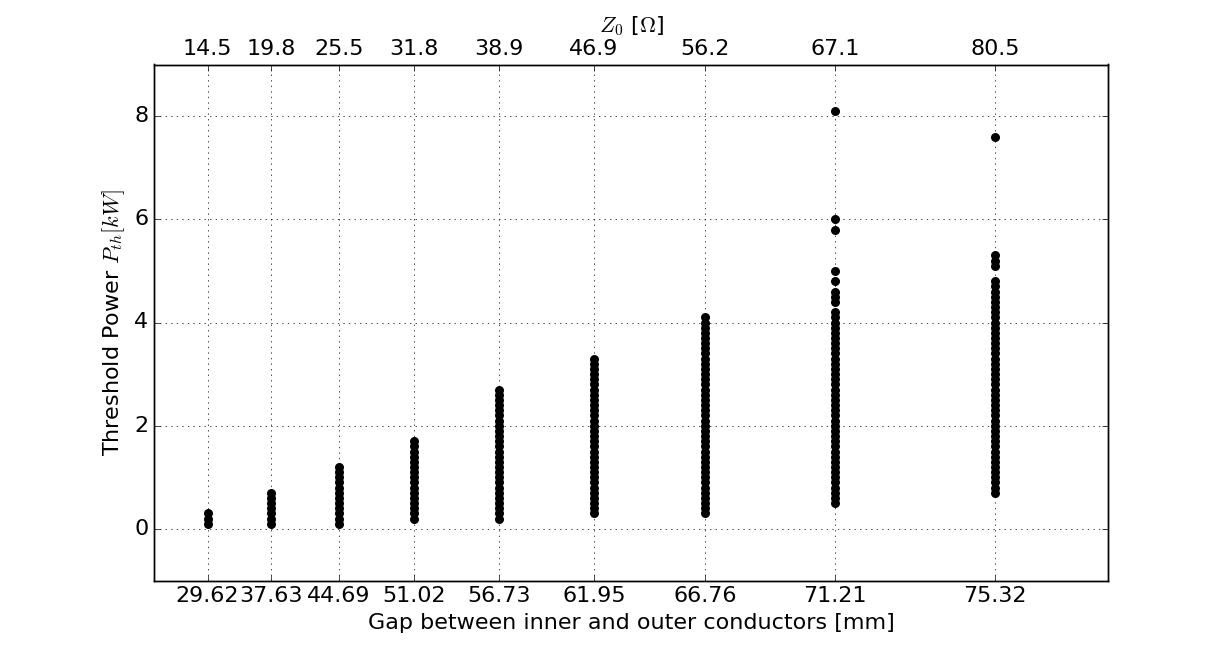
\includegraphics[width=1.0\linewidth]{figures/chap4/power_threshold_coax}
	\caption{Power Threshold in a coaxial line at 50 MHz calculated with Spark3D versus gap between inner and outer electrodes (with fixed outer diameter 153 mm) (Spark3D ECSS Copper SEY definition).}
	\label{fig:powerthresholdcoax}
\end{figure}


\subsection{Multipactor in LHRF}\label{sec:multipactor_lhrf}

LH Windows Multipactor
\sidecite{kim2007}

Vacuum arcs have been an experimental concern since the late 1970's \sidecite{ohkubo1977,timberlake1982}. Not only arcs can damage the components itself, but also they can release metallic impurities into the plasma (thus reducing the fusion power). While most arcs induce an increase of the reflected power, it some case however it can also remains unchanged or even decreases it.

The physical mechanism leading to these arcs is attributed to gas waveguide wall out-gassings, multipactor or photoelectron emission.

While the exact mechanism leading ultimately to arcs is barely fully certain, 

In the LHRF, multipactor has been early identified as a power-limiting mechanism in grill antennas. From the experience acquired on vacuum tubes, it has been suggested using slightly deformed waveguides, in order to introduce a certain electric field gradient which in returns can modify electron trajectories, might lead to multipactor suppression \sidecite{vaughan1982}. 

Surface treatment to decrease electron emission has been also tested in various experiments \sidecite{timberlake1982}. However, because of further surface changes appearing during component's life, such as chemical reactions with present species\footnote{Alcator C-Mod tokamak experienced chemical reactions between deuterium and a grill antenna made of titanium, which created a brittle titanium deuteride compound. The antenna disintegrated into titanium deuteride dust and the LH launcher was removed from the tokamak\cite{wallace2010}.} or surface erosion/deposition. Hence, such solution might be inherently less reliable on the long-term. 

Power limit and multipactor in grill:\cite{hwang1981, vaughan1982, goniche2012-2, goniche2014} 

removed with additionam agnetic field \sidecite{knowlton1982}
	
	
		


The analytical theory of multipactor in rectangular waveguide is detailled in  \sidecite{semenov2007-1}


\section{Influence of Magnetic Field on Secondary Emission}
\sidecite{becerra2007}





Dégradations des passages étanches des antennes FCI (origine?)
\sidecite{vulliez2007}







